% ==========================================================
\clearpage
\pagebreak
\justifying
\renewcommand{\thesection}{C \arabic{section}}

\titleformat{\section}{\normalfont\LARGE\bfseries\color{black}}{\thesection}{10pt}{\LARGE}
\section{Appendix-C3 Research Methodology}\label{sec:App3-Research-Methodology}

% ==========================================================
\subsection{App3-Pico Universal PWM Servo Controller}\label{sec:C-3.1-Universal PWM Servo Controller Board}
				
\begin{figure}[htbp]
	\begin{center}
		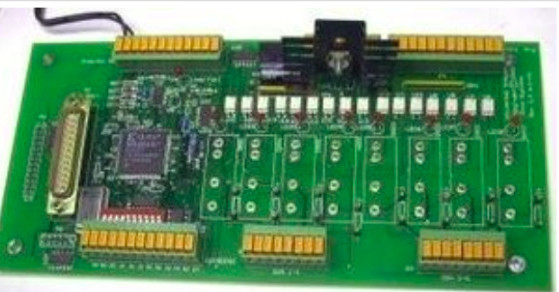
\includegraphics[width=0.85\textwidth]{./07-images/img-Ch3App/Universal-PWM-Servo-Controller.jpg}
		\caption{App3-Universal PWM Servo Controller Parallel Port Interface Board}
		\label{fig:App3-Universal-PWM-Servo-Controller.jpg}
	\end{center}
\end{figure}

\subsection{App3-Specifications Pico Universal PWM Servo Controller}

Reference: \url{http://www.pico-systems.com/motion.html}
\vspace{0.5cm}

The Universal PWM Servo Controller is a small board with everything needed to control a 2-axis, 3-axis or 4-axis machine tool with PWM-driven servo amplifiers. It contains 4 PWM generators with variable PWM drive frequency, 4 digital encoder counters to follow the machine position, 16 channels of opto-isolated digital inputs, and 8 positions for Solid State Relays of your choice to be mounted. It is connected to a computer by the parallel port. The parallel port must be at least capable of bi-directional exchange of data, but EPP or ECP modes give the best data transfer rate. The digital I/O section also implements emergency stop logic. There is an on board watchdog timer, which can be set to cause an emergency stop in case the computer fails to update the PWM generators in a timely fashion. This could shut off the servo amps, spindle motor, coolant, etc. For machines with more than 4 axes, 2 or more boards can be used together.
\vspace{0.5cm}

The computer reads the position from the encoder counters and computes a new PWM duty cycle to send to the PWM generators. This takes only about 50 uS on a 333 MHz Pentium II, so that reasonable servo update rates of 10 KHz could be made on such a machine. I usually use 1 KHz, because that is all that seems needed for machine-tool type applications.
\vspace{0.5cm}

The PWM generators divide a 10 MHz crystal clock by a minimum of 2 up to 216-1, which comes out to 5 MHz down to 153 Hz. A PWM frequency of 1 to 100 KHz is practical, and can be selected to suit the servo amplifiers. The duty cycle of the PWM waveform can be programmed in 100 nS steps, which is 1 percent at 100 KHz, but 0.2 percent at 20 KHz. The PWM and direction outputs can source or sink 12 mA to drive opto-coupled amplifier inputs.
\vspace{0.5cm}

The encoder counters keep a continuous watch over the encoder signals and can count up to 300,000 encoder counts/second, per channel. (The rev 5.x and later boards have an adjustable digital filter so that counting above 5 MHz can be performed.) They can also sense the index pulse from an encoder which has this feature. This can be used to more precisely locate the home position. If the encoder has no index channel, connect the index input (Z) to A.
\vspace{0.5cm}

The digital input section has 16 opto-isolators which can sense the condition of switches, relays, pressure switches, float sensors, etc. to allow the machine to be stopped if a fault condition occurs, sense when an axis is close to the travel limit or home position, etc. The board provides isolated 5V power to power the switches and/or sensors.
\vspace{0.5cm}

The digital output section provides sockets for up to 8 Opto-22 compatible Solid State Relays to be mounted directly onto the board. These sites are left unpopulated to allow the user to select SSRs with the output configuration and current capacity needed. A terminal strip is provided for connection to the outputs of the SSRs. LEDs monitor the command signal to each of the SSRs.
\vspace{0.5cm}

The last digital input is configured to monitor an emergency stop chain. A series circuit of normally-closed switches breaks the continuity of the circuit when an unsafe condition or problem develops (ie. spindle motor stall, servo amp overheat, lube level low, manual E-stop switch activated, etc.) An analog timer circuit can also monitor the flow of commands from the computer, and if the computer ceases updating the rate generators, then an E-stop can be caused. The E-stop condition turns off all signals to the solid state relays, as well as stopping the PWM generators, to bring the machine to a safe stop.
\vspace{0.5cm}

This boards contains a power regulator that produces all power needed by it from a provided 'wall-wart' type plug-in power supply.
\vspace{0.5cm}

The Universal PWM Controller takes advantage of the IEEE-1284 hardware signalling protocol, allowing multiple register addresses to be selected and transfers accomplished with minimum CPU overhead, and maximum data transfer rate. This requires a parallel port that can operate in the ECP or EPP mode. A male-female DB-25 cable specifically designed for IEEE-1284 compatability is required. Note: You MUST use a cable marked "IEEE-1284 compliant" for this system to work reliably.

% ==========================================================
\pagebreak
\subsection{App3-MCU Microchip 28-Pin LIN Development Board}\label{sec:C-3.3-MCU Microchip 28-Pin LIN Development Board}
				
\begin{figure}[htbp]
	\begin{center}
		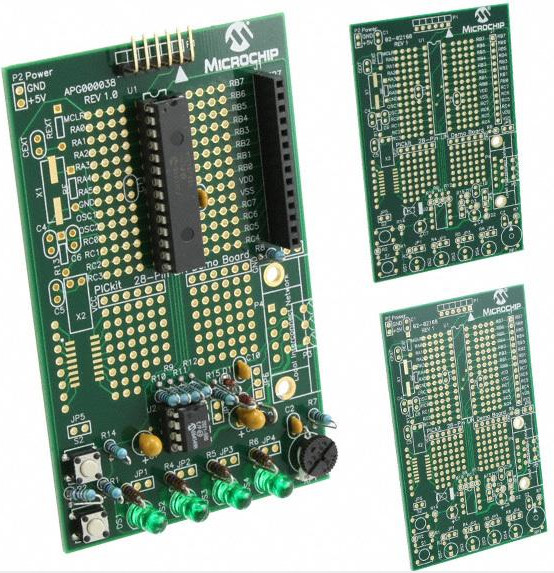
\includegraphics[width=0.95\textwidth]{./07-images/img-Ch3App/MCU-Microchip-Dev-Demo-Board.jpg}
		\caption{App3-MCU Microchip 28-Pin LIN Development Demo Interface Board}
		\label{fig:App3-MCU-Microchip-Dev-Demo-Board.jpg}
	\end{center}
\end{figure}

\subsection{App3-Specifications MCU Microchip 28-Pin LIN Development Board}

Reference: \url{https://www.digikey.my/products/en?keywords=DM164130-3-ND\%20\%20}\\
28-Pin LIN DEMO BOARD USER'S GUIDE\\
2009 Microchip Technology Inc.DSxxxxx\\
\vspace{0.5cm}

The 28-Pin LIN (Local Interconnect Network) Demo Board is a small and simple demonstration PCB for Microchip's 28-pin Dual Inline Package (DIP) PIC Microcontroller Units (MCU). It is populated with a PIC16F886 MCU, a MCP2021 LIN Transceiver with voltage regulator, four LEDs, 2 push buttons and a potentiometer. The demo board has several test points to access the I/O pins of the MCU and a generous prototyping area. The MCU can be programmed with the PICkit 2 Microcontroller Programmer or the MPLAB ICD 2 using the RJ-11 to 6-pin inline adapter (AC164110).
\vspace{0.5cm}

LIN (Local Interconnect Network) is an automotive networking technology, a sub-bus system based on a serial communications protocol. The bus is a single master/multiple slave bus that uses a single wire to transmit data.
\vspace{0.5cm}

The 28-Pin LIN Demo Board can be used with virtually any 28-pin Dual Inline Package (DIP) PIC MCU. The assembled 28-Pin LIN Demo Board is populated with a PIC16F886-I/P microcontroller. Additional 28-Pin LIN Demo Boards can be ordered from Microchip technology and distributors. Part number, DM164120-3, comes with one assembled and two blank 28-Pin LIN Demo Boards. 
\vspace{0.5cm}

The blank demo board can be used for evaluating or prototyping circuits using any of the 28-pin devices listed below.

\begin{figure}[htbp]
	\begin{center}
		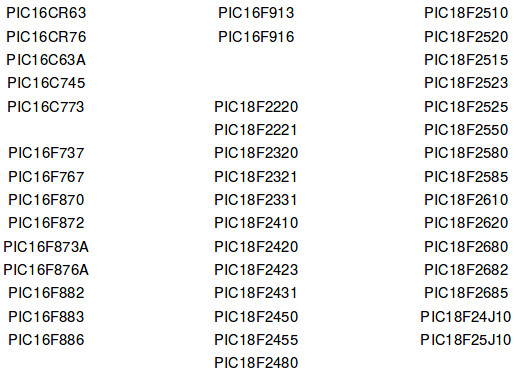
\includegraphics[width=0.85\textwidth]{./07-images/img-Ch3App/MCU-Chips-Supported-for-Dev-Demo-Board.jpg}
		\caption{App3-MCU Chips Supported-for Dev Demo Interface Board}
		\label{fig:App3-MCU-Chips-Supported-for-Dev-Demo-Board.jpg}
	\end{center}
\end{figure}

The 28-Pin LIN Demo Board is populated with a PIC16F886 MCU (U1), a MCP2021 LIN Transceiver with Voltage Regulator (U2), four LEDs (DS1-DS4), Two push buttons (SW1 and SW2), 32 KHz crystal (X2) and potentiometer (RP1). The board layout is shown in the figure below. The demo board has several test points to access the I/O pins of the MCU and a generous prototyping area. The MCU can be programmed with the PICkit 2 Microcontroller Programmer from header P1.
\vspace{0.5cm}

\pagebreak
\begin{figure}[htbp]
	\begin{center}
		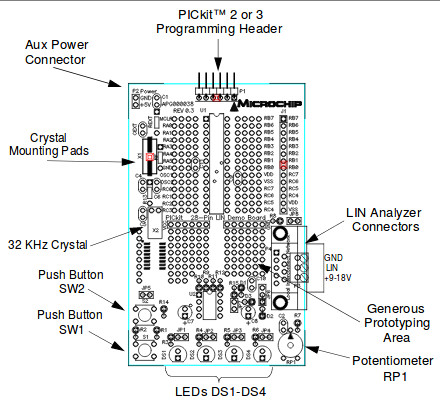
\includegraphics[width=0.95\textwidth]{./07-images/img-Ch3App/MCU-Microchip-28-Pin-LIN-Dev-Demo-Board.jpg}
		\caption{App3-MCU Microchip 28-Pin LIN Dev Demo Board Layout Diagram}
		\label{fig:App3-MCU-Microchip-28-Pin-LIN-Dev-Demo-Board.jpg}
	\end{center}
\end{figure}



% ==========================================================
\pagebreak
\subsection{App3-MCU Microchip Curiosity Development Board}\label{sec:C-3.5-Curiosity-Development-Board}

\begin{figure}[htbp]
	\begin{center}
		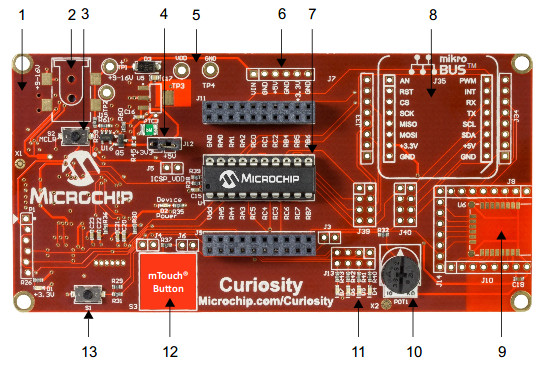
\includegraphics[width=0.85\textwidth]{./07-images/img-Ch3App/MCU-Curiosity-Dev-Board-Layout.jpg}
		\caption{App3-MCU Microchip Curiosity Demo Board Layout Diagram}
		\label{fig:App3-MCU-Curiosity-Dev-Board-Layout.jpg}
	\end{center}
\end{figure}
\begin{figure}[htbp]
	\begin{center}
		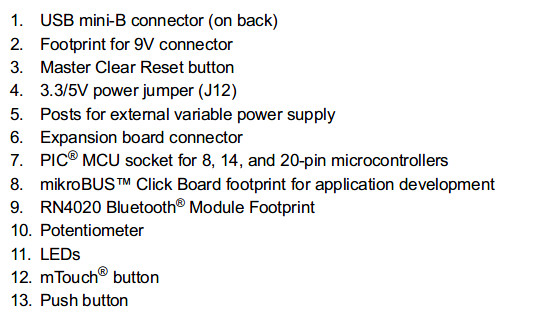
\includegraphics[width=0.65\textwidth]{./07-images/img-Ch3App/MCU-Curiosity-Dev-Board-Layout-Legend.jpg}
		\caption{App3-MCU Microchip Curiosity Demo Board Layout Legend}
		\label{fig:App3-MCU-Curiosity-Dev-Board-Layout-Legend.jpg}
	\end{center}
\end{figure}

\pagebreak
\subsection{App3-Specifications MCU Microchip Curiosity Development Board}
Reference: Curiosity Development Board User's Guide\\
2015-2016 Microchip Technology Inc. DS40001804B\\
\vspace{0.5cm}

The Curiosity Development Board supports Microchip's 8-pin, 14-pin and 20-pin 8-bit PIC MCUs. Dual-row expansion headers on either side of the socket offer flexibility of connectivity to all pins on the PIC MCUs. This board provides flexibility for 
experimentation through an application header with ground (GND) and supply voltage (VDD) connections. It also includes
a set of indication LEDs, mTouch button and push-button switches, and a variable potentiometer. Additionally, it features a 
Bluetooth low-energy footprint and a mikroBUS footprint to accommodate a variety of plug-in Click Board sensors that can be used in application development.
\vspace{0.5cm}

The Curiosity Development Board can be powered in one of three ways, depending on its usage.
\vspace{0.5cm}

\textbf{Power1 via USB Connector (J2)}\\

The USB connector (J2) will power the entire Curiosity Development Board. A shunt jumper must be placed onto jumper J12. The right two pins of J12 will connect +5V from the USB connector J2. The left two pins of J12 will connect +3.3V from the USB voltage regulator on the back side of the development board. With USB power connected to J2, power LED D1 will always be ON to indicate that +3.3V is available on the board. 
\vspace{0.5cm}

\textbf{Power2 via 9V External Power Supply (J15)}\\
%\vspace{0.5cm}

The 9V external power supply (J15) will also power the entire Curiosity Development Board. A shunt jumper must be placed onto jumper J12. The right two pins of J12 will connect +5V from the on-board voltage regulator circuitry connected to connector J15. The left two pins of J12 will connect +3.3V from the on-board voltage regulator circuitry. With 9V external power connected to J15, power LED D1 will always be ON to indicate that +3.3V is available on the board. Power LED D2 will only be ON when power (+3.3V or +5V) is applied to VDD via a shunt jumper placed on J12.
\vspace{0.5cm}

\textbf{Power3 via Variable External Power Supply (TP3, TP4)}\\
%\vspace{0.5cm}

A variable external power supply connected to TP3 and TP4 will power the entire Curiosity Development Board. A shunt jumper is not needed on J12, thus either +3.3V or +5V can be directly applied via a variable external power supply to VDD.
\vspace{0.5cm}


\textbf{Getting Started on Curiosity Board}\\
%\vspace{0.5cm}

The Curiosity Development Board must be used with MPLAB X Integrated Development Environment (IDE), available free on Microchip's web site, www.microchip.com. Use version v3.05 or later. The Curiosity Development Board, through MPLAB X, is a low-voltage in-circuit debugger, as well as a low-voltage programmer, for all supported devices. In-circuit debugging allows the user to run, examine and modify programs for the supported device embedded in the Curiosity hardware. This facilitates
the debugging of firmware and hardware concurrently. Use the Curiosity Development Board with MPLAB X IDE to run, stop and single-step through programs breakpoints can be set and the processor can be reset. When the processor stops, the contents of the register are available for examination and modification.
\vspace{0.5cm}

\textbf{Programming the Curiosity Board}\\
%\vspace{0.5cm}

After connecting the Curiosity Development Board to the computer using the on-board USB connector (J2 on the back of the board), open the MPLAB X IDE. Then create a new project or open an existing project. Click on the Project Properties icon located in the project's Dashboard window.
\vspace{0.5cm}

Alternatively, the Project Properties window can be opened by clicking on File, Project Properties, or by right-clicking on 
the project name in the Projects window and clicking Properties.
\vspace{0.5cm}

And it goes on.

% ==========================================================
